%%%%%%%%%%%%%%%%%%%%%%%%%%%%%%%%%%%%%%%%%%%%%%%%%%%%%%%%%%%%
%%  This Beamer template was created by Cameron Bracken.
%%  Anyone can freely use or modify it for any purpose
%%  without attribution.
%%
%%  Last Modified: January 9, 2009
%%

\documentclass[xcolor=x11names,compress]{beamer}

%% General document %%%%%%%%%%%%%%%%%%%%%%%%%%%%%%%%%%
\usepackage{graphicx}
\usepackage{tikz}
\usepackage[canadian]{babel}
\usepackage[utf8]{inputenc}
\usepackage{amsmath,amssymb}
\usepackage{mathtools}
\usepackage[ruled,vlined,linesnumbered]{algorithm2e}
\usepackage{epstopdf}
\usepackage{hyperref}
\usepackage[export]{adjustbox}
\usepackage{animate}
\usepackage{minted}
\usepackage{xcolor}
\usepackage{pgfplots}
\usetikzlibrary{calc}
\graphicspath{{img/}}
%%%%%%%%%%%%%%%%%%%%%%%%%%%%%%%%%%%%%%%%%%%%%%%%%%%%%%

\DeclareMathOperator*{\argmax}{arg\,max}
\DeclareMathOperator*{\argmin}{arg\,min}
%% Beamer Layout %%%%%%%%%%%%%%%%%%%%%%%%%%%%%%%%%%
\useoutertheme[subsection=false,shadow]{miniframes}
\useinnertheme{default}
\usefonttheme{serif}
\usepackage{palatino}
\urlstyle{same}
\setbeamerfont{title like}{shape=\scshape}
\setbeamerfont{frametitle}{shape=\scshape}

\setbeamercolor*{lower separation line head}{bg=DeepSkyBlue4} 
\setbeamercolor*{normal text}{fg=black,bg=white} 
\setbeamercolor*{alerted text}{fg=red} 
\setbeamercolor*{example text}{fg=black} 
\setbeamercolor*{structure}{fg=black} 
 
\setbeamercolor*{palette tertiary}{fg=black,bg=black!10} 
\setbeamercolor*{palette quaternary}{fg=black,bg=black!10} 

\renewcommand{\(}{\begin{columns}}
\renewcommand{\)}{\end{columns}}
\newcommand{\<}[1]{\begin{column}{#1}}
\renewcommand{\>}{\end{column}}
\setbeamertemplate{navigation symbols}{}

\setbeamerfont{footline}{size=\fontsize{6}{0}\selectfont}
\setbeamercolor{footline}{fg=black!50}

\setbeamertemplate{footline}{
	\parbox{\paperwidth}{\hspace*{5pt}\url{http://www.cs.toronto.edu/~frossard}\hfill
		\insertframenumber/\inserttotalframenumber\hspace*{5pt}}
	}
\usemintedstyle{tango}
%%%%%%%%%%%%%%%%%%%%%%%%%%%%%%%%%%%%%%%%%%%%%%%%%%

\begin{document}
%%%%%%%%%%%%%%%%%%%%%%%%%%%%%%%%%%%%%%%%%%%%%%%%%%%%%%
%%%%%%%%%%%%%%%%%%%%%%%%%%%%%%%%%%%%%%%%%%%%%%%%%%%%%%
\section{\scshape Introduction}
\begin{frame}
	\title{Introduction to Machine Learning}
	\subtitle{How Convolutional Neural Networks See}
	\author{
		Davi Frossard\\
		{\it Federal University of Espirito Santo \\ University of Toronto}\\
	}
	\date{
		\vspace{-2em}\\
		\includegraphics[width=0.6\columnwidth]{deepdream.jpg}\\[-1ex]
		\\
		\today
	}
	\titlepage
\end{frame}

%%%%%%%%%%%%%%%%%%%%%%%%%%%%%%%%%%%%%%%%%%%%%%%%%%%%%%
%%%%%%%%%%%%%%%%%%%%%%%%%%%%%%%%%%%%%%%%%%%%%%%%%%%%%%
\begin{frame}{Summary}
	\tableofcontents
\end{frame}

%%%%%%%%%%%%%%%%%%%%%%%%%%%%%%%%%%%%%%%%%%%%%%%%%%%%%%
%%%%%%%%%%%%%%%%%%%%%%%%%%%%%%%%%%%%%%%%%%%%%%%%%%%%%%
\begin{frame}{Introduction}
	\begin{itemize}
		\item Often neural networks are seen as black boxes.
		\item We may want to figure out what they are doing internally.
	\end{itemize}
\end{frame}

%%%%%%%%%%%%%%%%%%%%%%%%%%%%%%%%%%%%%%%%%%%%%%%%%%%%%%
%%%%%%%%%%%%%%%%%%%%%%%%%%%%%%%%%%%%%%%%%%%%%%%%%%%%%%
\section{\scshape Filters}
\begin{frame}{Filters}
	\begin{itemize}
		\item The most straightforward way to understand a ConvNet is by plotting its filters.
		\item We can easily extract the first
		\item<1-> Code:
		\begin{center}
			{\smaller \texttt{python visualize\_weights.py}}
		\end{center}
	\end{itemize}
\end{frame}

%%%%%%%%%%%%%%%%%%%%%%%%%%%%%%%%%%%%%%%%%%%%%%%%%%%%%%
%%%%%%%%%%%%%%%%%%%%%%%%%%%%%%%%%%%%%%%%%%%%%%%%%%%%%%
\begin{frame}{Filters}
	\begin{center}
		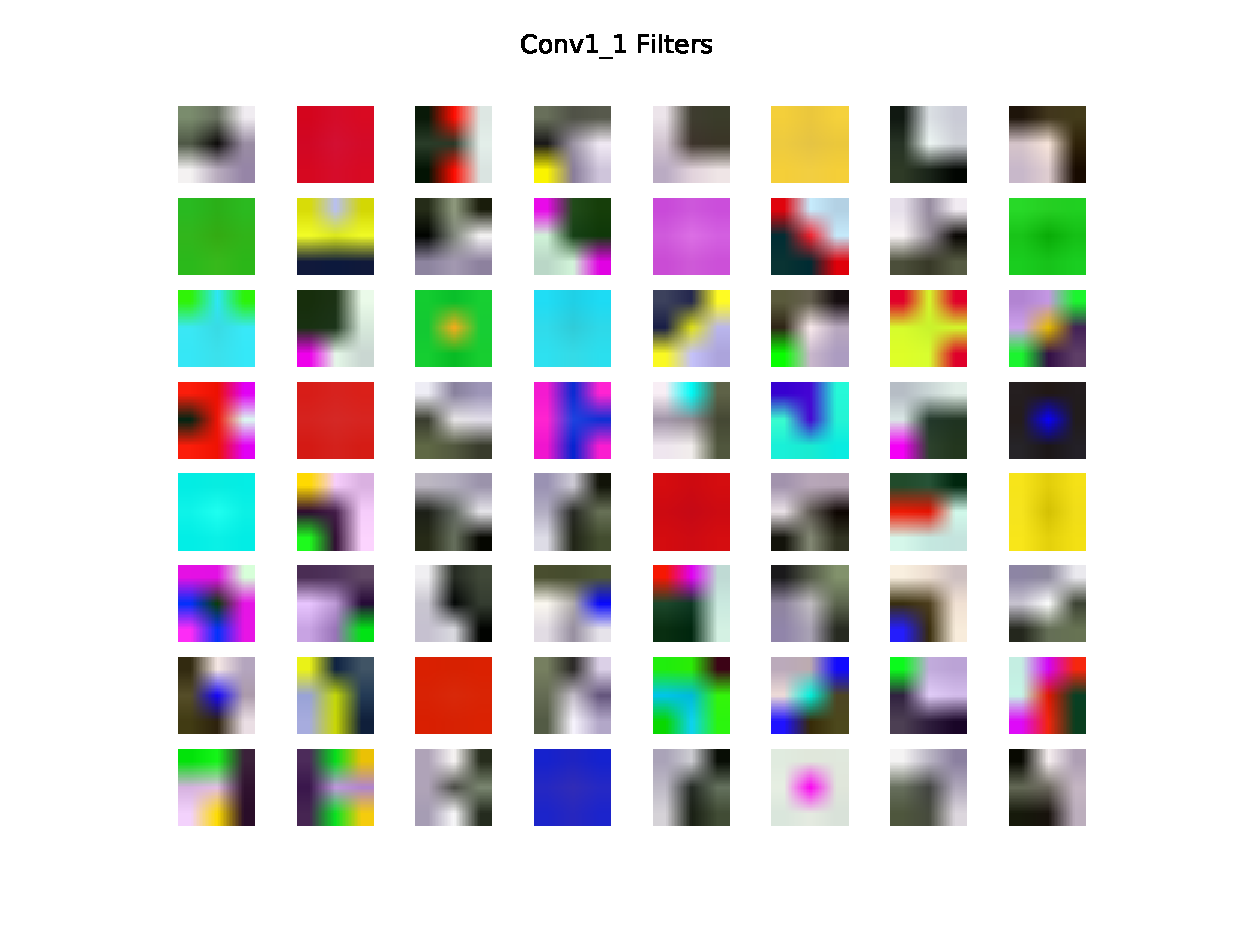
\includegraphics[width=\columnwidth,trim={0cm 0cm 0 1cm},clip]{weights.eps}
	\end{center}
\end{frame}

%%%%%%%%%%%%%%%%%%%%%%%%%%%%%%%%%%%%%%%%%%%%%%%%%%%%%%
%%%%%%%%%%%%%%%%%%%%%%%%%%%%%%%%%%%%%%%%%%%%%%%%%%%%%%
\begin{frame}{Filters}
	\begin{itemize}
		\item Unsurprisingly, they extract very simple features from the images.
		\item Plotting the weights from the upper layers is possible, but becomes increasingly boring.
		\item We want a general way of visualizing the ConvNet.
	\end{itemize}
\end{frame}

%%%%%%%%%%%%%%%%%%%%%%%%%%%%%%%%%%%%%%%%%%%%%%%%%%%%%%
%%%%%%%%%%%%%%%%%%%%%%%%%%%%%%%%%%%%%%%%%%%%%%%%%%%%%%
\section{\scshape Data Driven}
\begin{frame}{Data Driven}
	\begin{itemize}
		\item The data driven approach consists in using lots of data to infer the network behavior.
		\item We can feed a large dataset to a model and keep track of the images that maximally activate some neuron.
		\item This gives us a sense of what the neuron is looking for.
	\end{itemize}
\end{frame}

%%%%%%%%%%%%%%%%%%%%%%%%%%%%%%%%%%%%%%%%%%%%%%%%%%%%%%
%%%%%%%%%%%%%%%%%%%%%%%%%%%%%%%%%%%%%%%%%%%%%%%%%%%%%%
\begin{frame}{Data Driven}
	\begin{center}
		\includegraphics[width=\columnwidth]{pool5max.jpeg}\\[-1ex]
		{\tiny Credit: {\itshape \url{http://cs231n.github.io/understanding-cnn/}}}
	\end{center}
\end{frame}

%%%%%%%%%%%%%%%%%%%%%%%%%%%%%%%%%%%%%%%%%%%%%%%%%%%%%%
%%%%%%%%%%%%%%%%%%%%%%%%%%%%%%%%%%%%%%%%%%%%%%%%%%%%%%
\begin{frame}{Data Driven}
	\begin{itemize}
		\item Additionally, we can slide an occlusion window through the input image and keep track of how the ground truth label score behaves.
		\item We then plot a heatmap and determine the network's region of interest.
	\end{itemize}
\end{frame}

%%%%%%%%%%%%%%%%%%%%%%%%%%%%%%%%%%%%%%%%%%%%%%%%%%%%%%
%%%%%%%%%%%%%%%%%%%%%%%%%%%%%%%%%%%%%%%%%%%%%%%%%%%%%%
\begin{frame}{Data Driven}
	\begin{center}
		\includegraphics[width=\columnwidth]{occlude.jpeg}\\[-1ex]
		{\tiny Credit: {\itshape \url{http://cs231n.github.io/understanding-cnn/}}}
	\end{center}
\end{frame}

%%%%%%%%%%%%%%%%%%%%%%%%%%%%%%%%%%%%%%%%%%%%%%%%%%%%%%
%%%%%%%%%%%%%%%%%%%%%%%%%%%%%%%%%%%%%%%%%%%%%%%%%%%%%%
\section{\scshape Gradient}
\begin{frame}{Gradient}
	\begin{itemize}
		\item A numerical alternative to the data driven approach is to use gradients.
		\item If we take the gradient of an output neuron with respect to the input image,
		we will be seeing which neurons need to change the least to affect the output the most.
		\item Because the softmax outputs take into account not only the positive evidence but also all the negative evidence, looking at the unscaled logits may give a better view.
		\item<2-> Code:
		\begin{center}
			{\smaller \texttt{python gradient.py}}
		\end{center}
	\end{itemize}
\end{frame}

%%%%%%%%%%%%%%%%%%%%%%%%%%%%%%%%%%%%%%%%%%%%%%%%%%%%%%
%%%%%%%%%%%%%%%%%%%%%%%%%%%%%%%%%%%%%%%%%%%%%%%%%%%%%%
\begin{frame}{Gradient}
	\begin{center}
		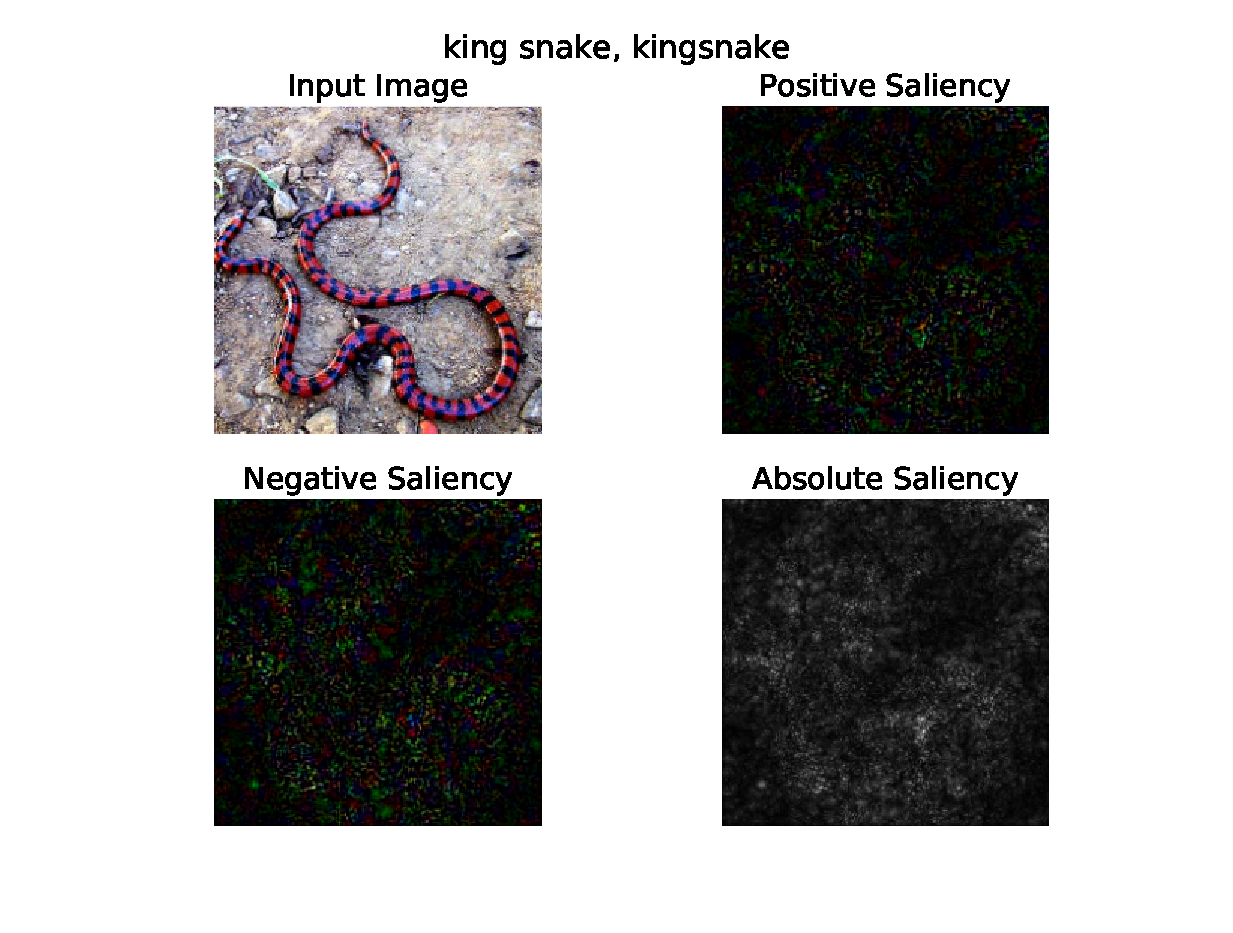
\includegraphics[width=\columnwidth]{gradients.eps}
	\end{center}
\end{frame}

%%%%%%%%%%%%%%%%%%%%%%%%%%%%%%%%%%%%%%%%%%%%%%%%%%%%%%
%%%%%%%%%%%%%%%%%%%%%%%%%%%%%%%%%%%%%%%%%%%%%%%%%%%%%%
\begin{frame}{Gradient}
	\begin{itemize}
		\item The gradients look convoluted, roughly showing which pixels affect the output the most.
		\item One issue is that at each gradient step both the neurons positively and negatively correlated with the output are taken into account.
		\item This makes it harder to visualize what the network is doing.
	\end{itemize}
\end{frame}

%%%%%%%%%%%%%%%%%%%%%%%%%%%%%%%%%%%%%%%%%%%%%%%%%%%%%%
%%%%%%%%%%%%%%%%%%%%%%%%%%%%%%%%%%%%%%%%%%%%%%%%%%%%%%
\section{\scshape Guided Backpropagation}
\begin{frame}{Guided Backpropagation}
	\begin{itemize}
		\item To extract different gradients for the positively and negatively correlated neurons we have Guided Backpropagation.
		\item Instead of using the actual gradient of the neurons, we zero out the entries where either the incoming our outgoing gradient is negative.
		\item This effectively prevents the backward flow of data from neurons which decrease the activation of the layer we're looking at.
	\end{itemize}
\end{frame}

%%%%%%%%%%%%%%%%%%%%%%%%%%%%%%%%%%%%%%%%%%%%%%%%%%%%%%
%%%%%%%%%%%%%%%%%%%%%%%%%%%%%%%%%%%%%%%%%%%%%%%%%%%%%%
\begin{frame}{Guided Backpropagation}
	\begin{itemize}
		\item If we have an error signal $\delta_i$, its backward flow through a ReLU layer will be:
		\begin{gather*}
			\delta_{i-1} = \delta_i \cdot [x>0]
		\end{gather*}
		\item Guided backpropagation proposes we only retain positive signals, therefore:
		\begin{gather*}
			\delta_{i-1} = \delta_i \cdot [x>0] \cdot [\delta_i > 0]
		\end{gather*}
		\item<2-> Code:
		\begin{center}
			{\smaller \texttt{python guided\_backpropagation.py}}
		\end{center}
	\end{itemize}
\end{frame}

%%%%%%%%%%%%%%%%%%%%%%%%%%%%%%%%%%%%%%%%%%%%%%%%%%%%%%
%%%%%%%%%%%%%%%%%%%%%%%%%%%%%%%%%%%%%%%%%%%%%%%%%%%%%%
\begin{frame}{Guided Backpropagation}
	\begin{center}
		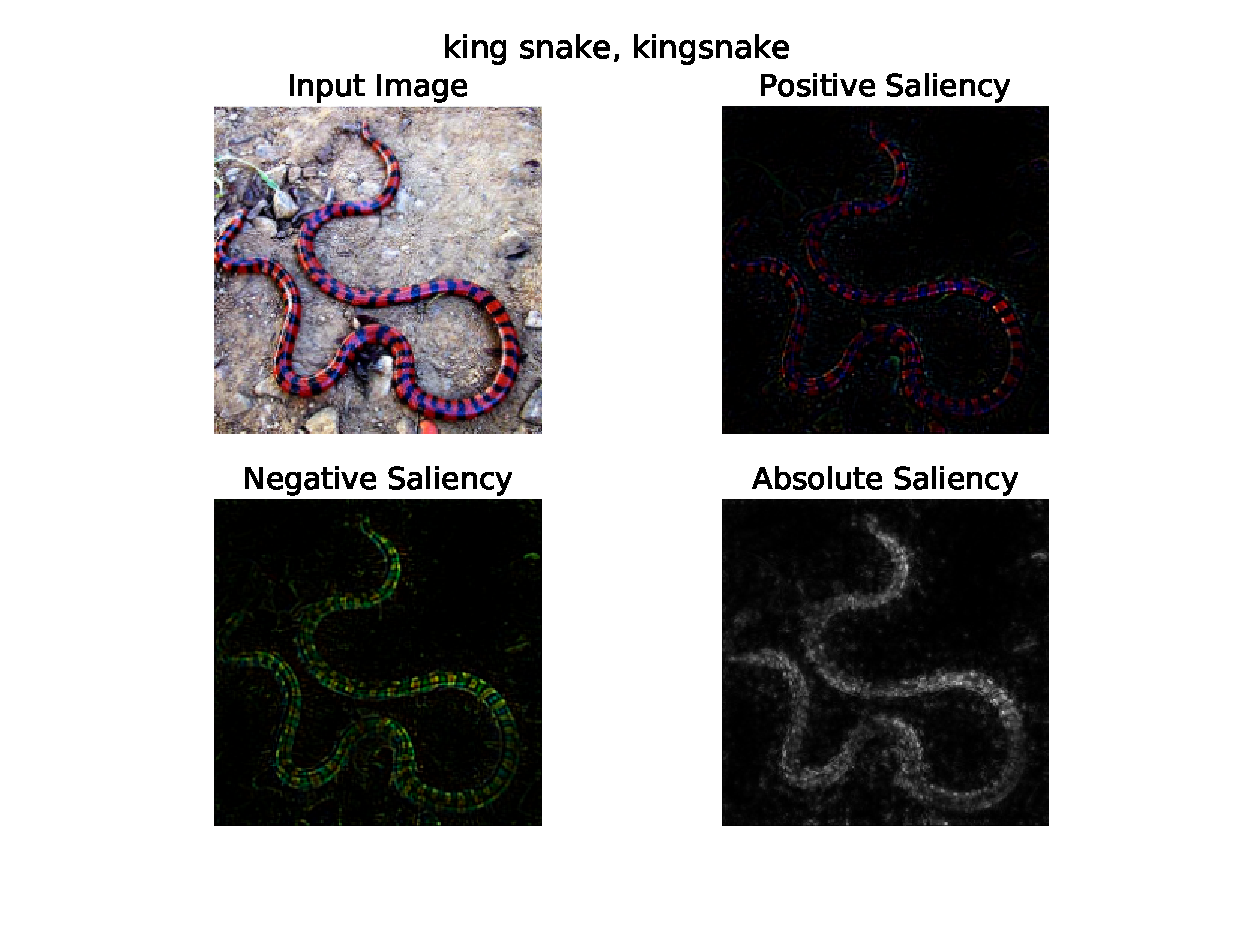
\includegraphics[width=\columnwidth]{guided_backprop.eps}
	\end{center}
\end{frame}

%%%%%%%%%%%%%%%%%%%%%%%%%%%%%%%%%%%%%%%%%%%%%%%%%%%%%%
%%%%%%%%%%%%%%%%%%%%%%%%%%%%%%%%%%%%%%%%%%%%%%%%%%%%%%
\section{\scshape Gradient Ascent}
\begin{frame}{Gradient Ascent}
	\begin{itemize}
		\item Following the idea of using gradients, we could actually "train" the image with this information and maximize a certain activation.
		\item We start with a plain image (with some noise for symmetry breaking) and perform gradient ascent.
		\item<2-> Code:
		\begin{center}
			{\smaller \texttt{python naive\_filter.py}}
		\end{center}
	\end{itemize}
\end{frame}

%%%%%%%%%%%%%%%%%%%%%%%%%%%%%%%%%%%%%%%%%%%%%%%%%%%%%%
%%%%%%%%%%%%%%%%%%%%%%%%%%%%%%%%%%%%%%%%%%%%%%%%%%%%%%
\begin{frame}{Gradient Ascent}
	\begin{center}
		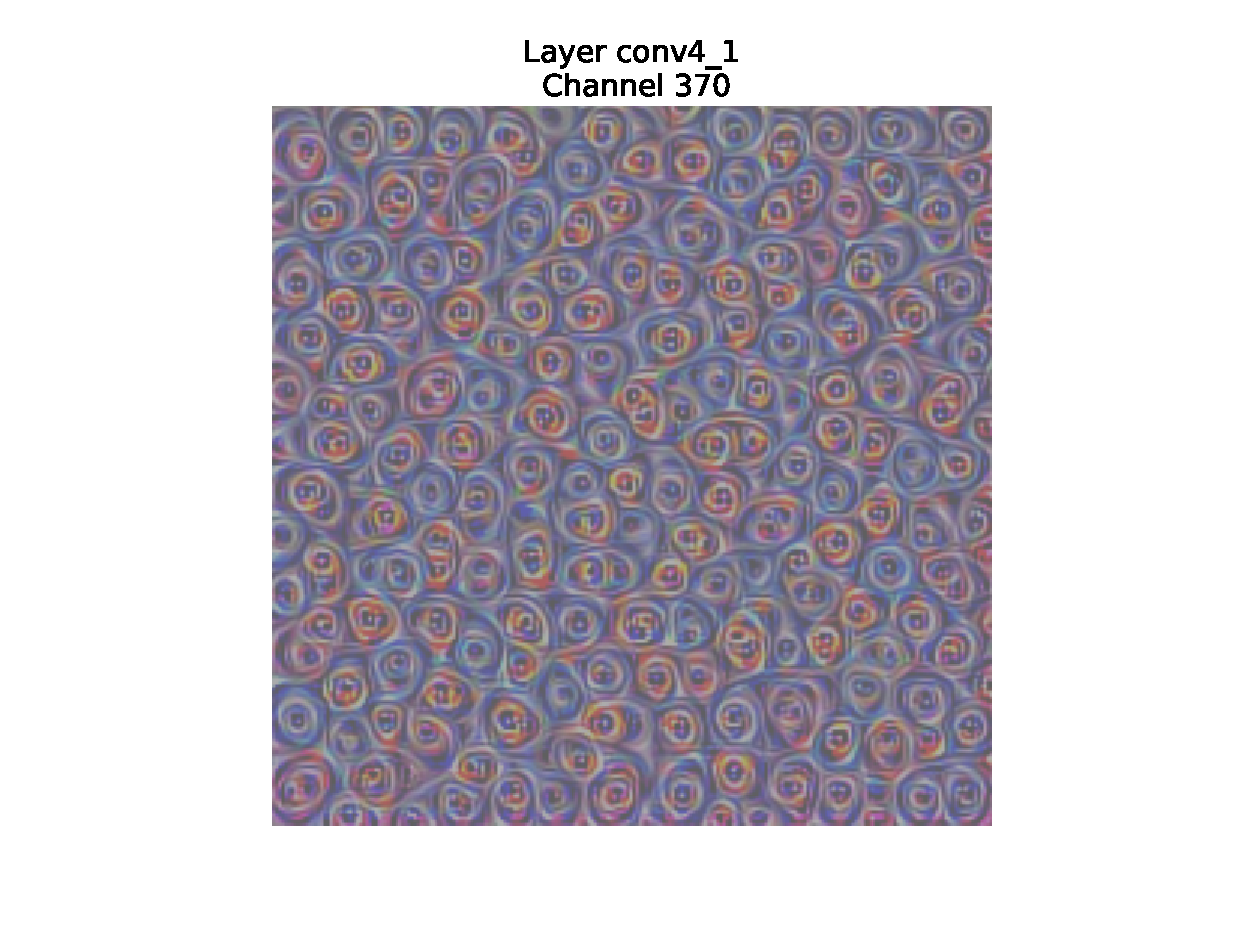
\includegraphics[width=\columnwidth]{naive_filter.eps}
	\end{center}
\end{frame}

%%%%%%%%%%%%%%%%%%%%%%%%%%%%%%%%%%%%%%%%%%%%%%%%%%%%%%
%%%%%%%%%%%%%%%%%%%%%%%%%%%%%%%%%%%%%%%%%%%%%%%%%%%%%%
\section{\scshape Deep Dream}
\begin{frame}{Deep Dream}
	\begin{itemize}
		\item With clever modifications to the previous approach, we can tune an image to
		look more and more like some objects that were \textit{kind of} detected at first.
		\begin{itemize}
			\item Select a layer and \textit{make the rich get richer.}
			\item Update the input such that the neurons with the highest activations get higher.
			\item This can be achieved by multiplying the gradient by the normalized activation map.
		\end{itemize}
	\end{itemize}
\end{frame}

%%%%%%%%%%%%%%%%%%%%%%%%%%%%%%%%%%%%%%%%%%%%%%%%%%%%%%
%%%%%%%%%%%%%%%%%%%%%%%%%%%%%%%%%%%%%%%%%%%%%%%%%%%%%%
\begin{frame}{Deep Dream}
	\begin{itemize}
		\item As it is, this wouldn't produce visually pleasing images.
		\begin{itemize}
			\item The gradient would keep being applied on the same areas over and over again. Creating saturated features and not much diversity.
			\item We are also constrained to use images only as big as the ConvNet input.
		\end{itemize}
		\item We can solve this by applying the gradient over random tiles of the image.
		\begin{itemize}
			\item Sample a tile of the image with the same size as the ConvNet input and backpropagate over that region.
			\item Through the iterations, this discretization gets smoothed.
		\end{itemize}
	\end{itemize}
\end{frame}

%%%%%%%%%%%%%%%%%%%%%%%%%%%%%%%%%%%%%%%%%%%%%%%%%%%%%%
%%%%%%%%%%%%%%%%%%%%%%%%%%%%%%%%%%%%%%%%%%%%%%%%%%%%%%
\begin{frame}{Deep Dream}
	\begin{itemize}
		\item We can make the output extra nicer by "training" over different scales (octaves).
		\begin{itemize}
			\item Generate multiple resolutions of the same image and accumulate the results over each octave.
		\end{itemize}
		\item<2-> Code:
		\begin{center}
			{\smaller \texttt{python deep\_dream.py}}
		\end{center}
	\end{itemize}
\end{frame}

%%%%%%%%%%%%%%%%%%%%%%%%%%%%%%%%%%%%%%%%%%%%%%%%%%%%%%
%%%%%%%%%%%%%%%%%%%%%%%%%%%%%%%%%%%%%%%%%%%%%%%%%%%%%%
\begin{frame}{Deep Dream}
	\begin{center}
		\includegraphics[width=0.9\columnwidth]{../Sample_Code/sky.jpg}
	\end{center}
\end{frame}

%%%%%%%%%%%%%%%%%%%%%%%%%%%%%%%%%%%%%%%%%%%%%%%%%%%%%%
%%%%%%%%%%%%%%%%%%%%%%%%%%%%%%%%%%%%%%%%%%%%%%%%%%%%%%
\begin{frame}{Deep Dream}
	\begin{center}
		\includegraphics[width=0.9\columnwidth]{dd_sky.jpg}
	\end{center}
\end{frame}

%%%%%%%%%%%%%%%%%%%%%%%%%%%%%%%%%%%%%%%%%%%%%%%%%%%%%%
%%%%%%%%%%%%%%%%%%%%%%%%%%%%%%%%%%%%%%%%%%%%%%%%%%%%%%
\begin{frame}{Addendum}
	\begin{itemize}
		\item We can use gradient ascent to create images that look nothing like a class, yet score highly (99.9\% certainty).
	\end{itemize}
	\begin{center}
		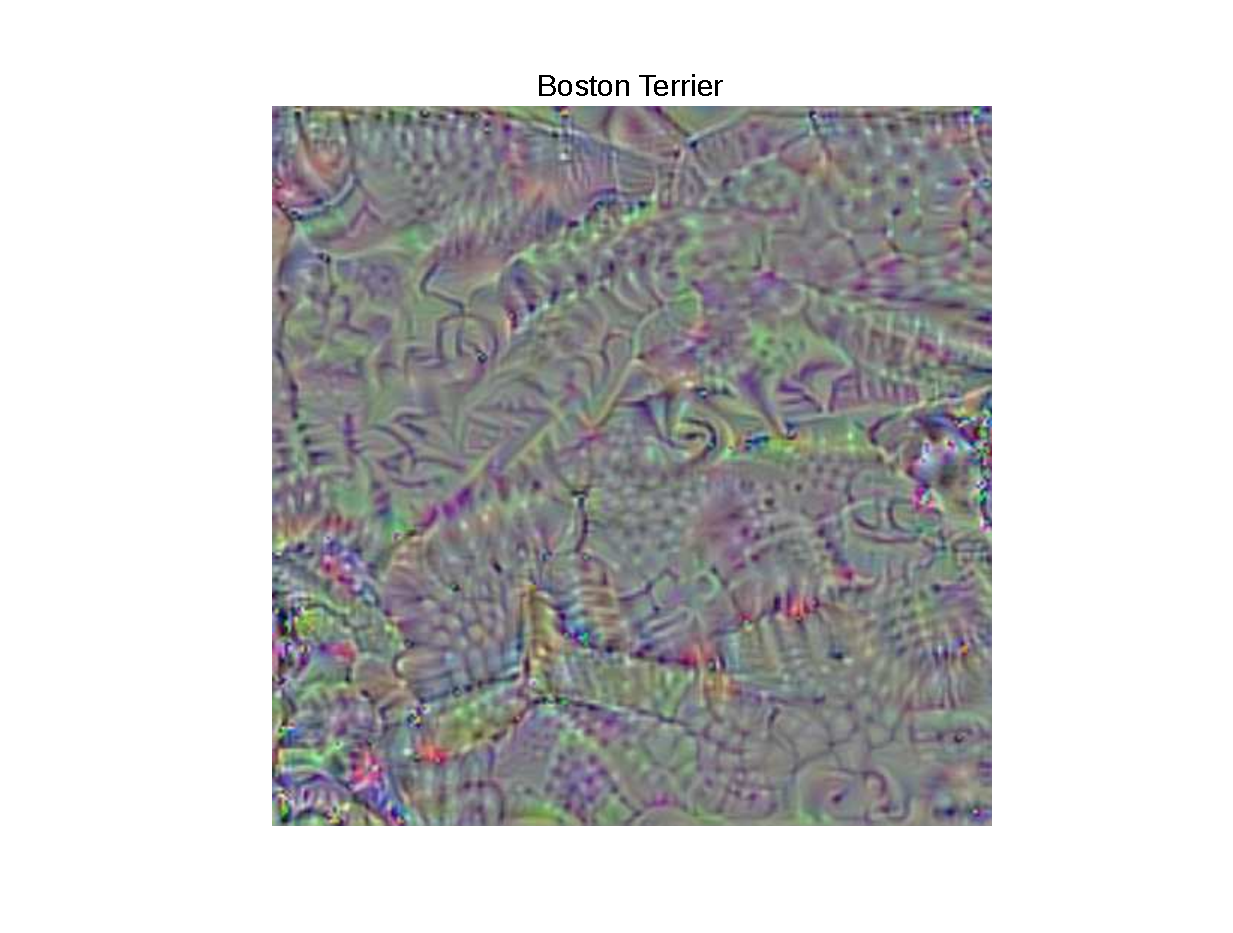
\includegraphics[width=0.85\columnwidth]{boston_terrier.eps}
	\end{center}
\end{frame}

\end{document}
